%%%%%%%%%%%%%%%%%%%%%%%%%%%%
% SECTION                  %
%%%%%%%%%%%%%%%%%%%%%%%%%%%%
\vspace{1em}

Après la finalisation du programme précédemment analysé, de nouveaux entretiens avec Bruno VALENTIN et Sébastien ABBONDANZA ont eu lieu afin de réfléchir aux améliorations à mettre en place durant le temps restant de mon stage.\\

Nos réflexions sur l'état actuel du système nous ont amenés à estimer que le nombre de sources de CTI de l'AMSN était trop faible pour garantir la capacité des sondes à détecter toutes les menaces pertinentes et existantes à l'état de l'art. Aussi, cette observation nous a conduits à envisager l'intégration de nouvelles sources de renseignements cyber pour mon programme et plus largement pour l'Agence.\\

Notre choix s'est porté sur l'intégration et l'exploitation d'une instance MISP\footnote{Malware Information Sharing Platform and Threat Sharing : \url{https://www.misp-project.org/}}, qui est une plateforme collaborative de partage d'informations, conçue pour améliorer la détection et la prévention des incidents de sécurité. Ce projet open source a été initié par l’équipe de sécurité du CIRCL\footnote{Centre Gouvernemental de Cyberdéfense du Luxembourg : \url{https://www.circl.lu/}} afin d'encourager la collaboration internationale de lutte contre les cybermenaces.\\

La plateforme MISP est utilisée par des organisations du monde entier, notamment des agences gouvernementales, des entreprises privées, des équipes de réponse aux incidents de sécurité (CSIRT/CERT), ainsi que des chercheurs en cybersécurité. Les informations partagées via MISP sont partiellement publiques, en effet, une partie, à laquelle l'AMSN a le droit d'accéder, est confidentielle et partagée uniquement entre partenaires de confiance.\\

\vspace{1em}

\subsubsection{\textit{Note}}
Il existe de nombreuses solutions de partage de renseignements (OpenCTI, alienvault, etc.) mais MISP nous a semblé être le choix le plus approprié car il s'agit d'une des plateformes les plus utilisées et qui permet de centraliser des informations provenant des autres outils. De plus, les partenaires de l'Agence (notamment l'ANSSI) s'appuient déjà sur cet outil pour partager des "feed"\footnote{\url{https://misp.cert.ssi.gouv.fr/feed-misp/}} d'information.

\newpage

\subsection{Fonctionnement de MISP}

L'échange d'informations entre entités utilisatrices de MISP se réalise via la création d'évènements qui sont partagés entre les instances locales de MISP dont bénéficient les différentes organisations. A titre d'exemple, ce processus peut prendre cette forme :\\

\vspace{1em}

\begin{figure}[h]%
    \center%
    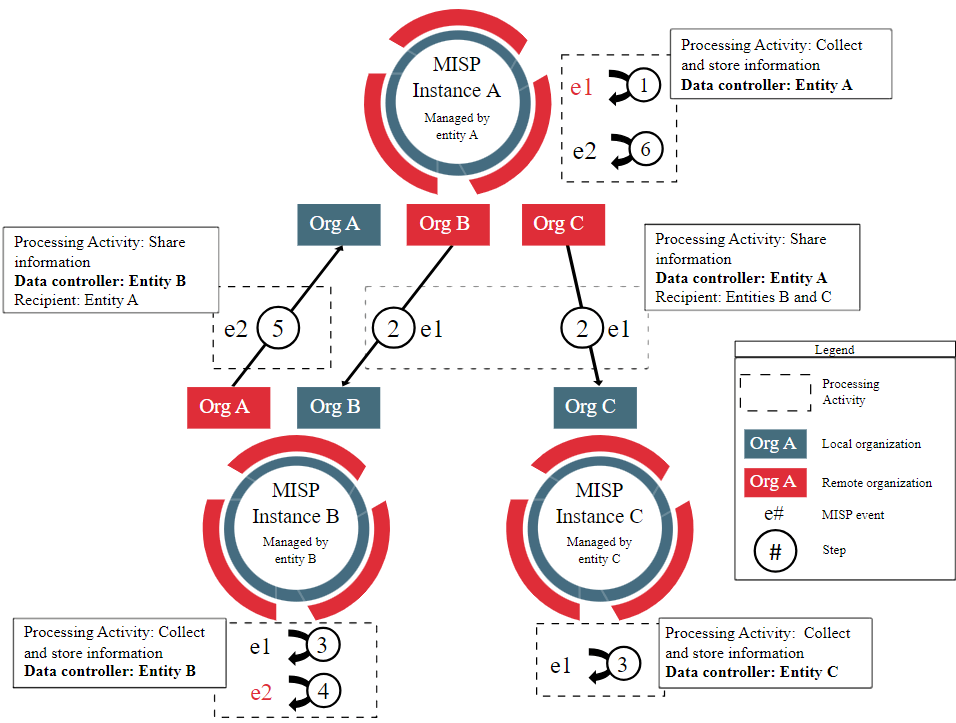
\includegraphics[width=0.8\textwidth]{assets/misp-compliance-gdpr.png}
    \caption[Démonstration de l'échange d'informations entre entités via MISP (source: \href{https://www.misp-project.org/compliance/GDPR/}{www.misp-project.org})]{Démonstration de l'échange d'informations entre entités via MISP}\label{fig:misp-compliance-gdpr}
\end{figure}

\vspace{1em}

\begin{itemize}[itemsep=0.8em]
    \item[•] \textbf{1 :} Un événement MISP "\textbf{e1}" est créé par l'entité \textbf{A}.
    \item[•] \textbf{2 :} L'entité \textbf{A} décide de partager l'événement avec des organisations distantes partenaires (entités \textbf{B} et \textbf{C}).
    \item[•] \textbf{3 :} Les entités \textbf{B} et \textbf{C} stockent l'événement "\textbf{e1}" dans leur instance locale de MISP.
    \item[•] \textbf{4 :} L'entité \textbf{B} crée un second événement "\textbf{e2}".
    \item[•] \textbf{5 :} L'entité \textbf{B} décide de ne partager "\textbf{e2}" qu'avec l'entité \textbf{A}.
    \item[•] \textbf{6 :} L'entité \textbf{A} stocke l'événement "\textbf{e2}".\\
\end{itemize}

\newpage

\label{chap3:mispEvents}
Un événement MISP est un ensemble structuré d'informations relatives à un incident, une menace ou une observation spécifique en matière de cybersécurité, qui est géré au sein de la plateforme MISP. Ces événements permettent d'organiser et de partager des informations détaillées sur divers types de cybermenaces, notamment les attaques de logiciels malveillants, les tentatives d'hameçonnage, les vulnérabilités et d'autres incidents de sécurité. Chaque événement MISP peut inclure plusieurs attributs et indicateurs de compromission (IOC) qui permettent de comprendre la menace et d'être capable de la détecter à nouveau. Un événement MISP se compose principalement des éléments suivants :\\

\begin{itemize}[itemsep=1em]
    \item[•] \textbf{\textit{Attributes} :} Il s'agit de données individuelles qui décrivent des caractéristiques spécifiques de l'événement. Les attributs peuvent inclure des adresses IP, des noms de domaine, des hachages de fichiers, des adresses électroniques, des URL, des échantillons de logiciels malveillants et d'autres détails techniques qui permettent d'identifier et d'analyser la menace.
    \item[•] \textbf{\textit{Tags} :} Les "Tags" sont utilisés pour classer et étiqueter les événements afin de faciliter la recherche et le filtrage. Les étiquettes peuvent inclure des classifications telles que "phishing", "APT" (Advanced Persistent Threat), "malware" ou "ransomware", ainsi que des informations sur la sensibilité ou les exigences de traitement des données.
    \item[•] \textbf{\textit{Objects} :} Ce sont des groupes d'attributs liés qui, ensemble, décrivent des entités ou des scénarios plus complexes, tels qu'une personne, un courrier électronique ou un périphérique de réseau. Cela permet de fournir un contexte et une structure aux données.
    \item[•] \textbf{\textit{Relations }:} Les événements peuvent être liés à d'autres événements ou objets pour indiquer les relations entre différents incidents, ce qui permet aux utilisateurs de voir les connexions et les corrélations qui ne sont pas toujours évidentes.
    \item[•] \textbf{\textit{Comments }:} Les utilisateurs peuvent ajouter des commentaires à un événement pour fournir un contexte, une analyse ou des recommandations supplémentaires, ce qui facilite la collaboration et le partage des connaissances entre les analystes.
    \item[•] \textbf{\textit{Threat Level/Analysis} :} Les événements comprennent souvent un indicateur de niveau de menace et de niveau d'avancement de l'analyse de l'événement (faible, moyen, élevé), qui peut aider à hiérarchiser la réponse à des menaces spécifiques.\\
\end{itemize}

\newpage

\begin{figure}[h]%
    \center%
    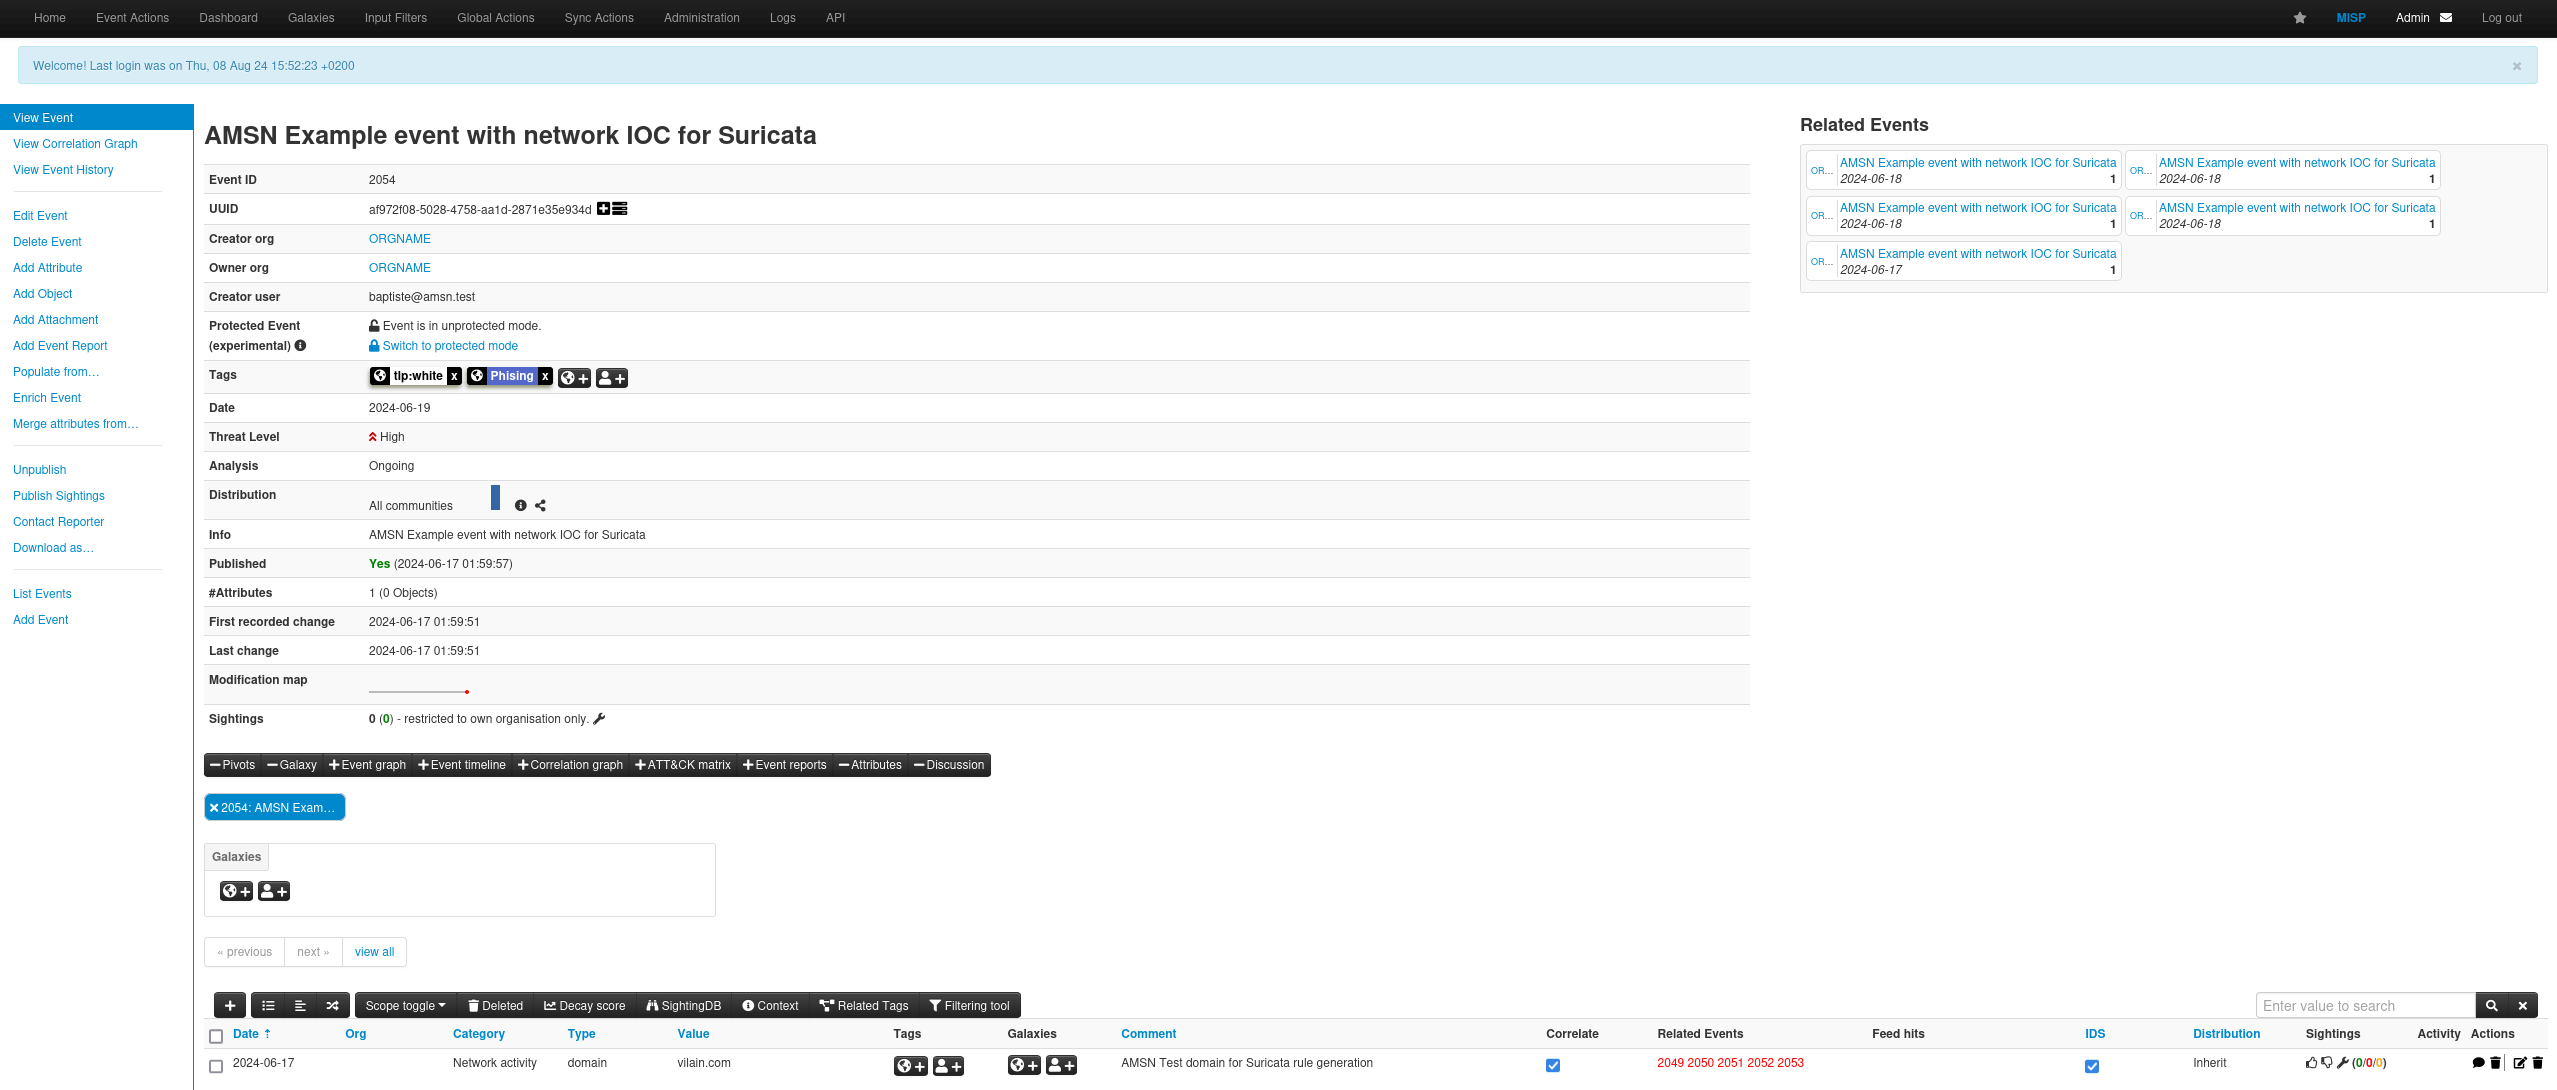
\includegraphics[width=1\textwidth]{assets/CaptureMisp.png}
    \caption[Exemple d'événement MISP (source : capture d'écran de l'interface graphique de l'instance de test locale MISP)]{Exemple d'événement MISP (source : capture d'écran de l'interface graphique de l'instance de test locale MISP)}\label{fig:CaptureMisp}
\end{figure}

\vspace{1em}

Parmi ces éléments, les plus importants pour répondre à notre problématique sont les \textit{Attributes} et les \textit{Objects} (qui sont des ensembles d'\textit{Attributes}), lesquels contiennent les éléments d'identification uniques des événements qui peuvent être utilisés pour créer des IOC, les autres servant principalement d'éléments de contexte et d'explication de l'événement. Dans ces \textit{Attributes}, je vais extraire les IOC compatibles avec Suricata (adresses IP, noms de domaine, URL, hachages de fichiers et User-Agent), afin de les transformer automatiquement en règles de détection qui seront ajoutées à notre ensemble de règles envoyées aux sondes.\\

\subsubsection{\textit{Note}}
J'ai également eu l'occasion d'effectuer quelques tâches supplémentaires avec MISP afin de soutenir le SOC-MC au quotidien. Les analystes du SOC m'avaient fait part de leur difficulté à comprendre certaines règles envoyées sans contexte par les partenaires. MISP m'a permis de répondre en partie à cette difficulté en offrant la possibilité de contextualiser les règles qui génèrent des alertes à partir d'événements sur le MISP partageant les mêmes IOC. Cependant, ce travail sort du cadre de ma problématique, voire est négligeable par rapport à l'ensemble de mon travail, je n'y reviendrai donc pas dans la suite de ce document.

\newpage

\subsection{Exploitation de MISP}

\vspace{1em}

La première étape de l'intégration de MISP dans le processus de mise à jour des règles a consisté à installer une VM (machine virtuelle), dans le réseau interne de l'Agence, à l'aide des guides fournis par le CIRCL\footnote{\url{https://misp.github.io/MISP/}}. Pour la tenir à jour avec les derniers événements partagés sur le réseau MISP sans avoir à exposer notre instance locale, j'ai utilisé MISP Guard\footnote{un addon mitmproxy développé par l'équipe qui est à l'origine de MISP : \url{https://www.misp-project.org/2022/09/13/misp-guard.html/}} qui permet de créer un proxy capable de récupérer les mises à jour de manière sécurisée sans menacer notre instance locale ou notre réseau interne.\\

\vspace{1em}

\begin{figure}[h]%
    \center%
    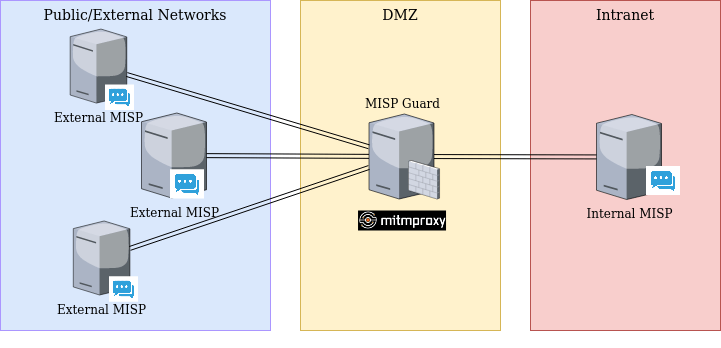
\includegraphics[width=0.85\textwidth]{assets/MispGard.png}
    \caption[Installation sécurisée de MISP dans le réseau de l'Agence (source: \url{https://www.misp-project.org/img/blog/misp-guard-architecture.png})]{Installation sécurisée de MISP dans le réseau de l'Agence}\label{fig:MispGard}
\end{figure}

L'instance locale de MISP est utilisée systématiquement via l'API. Mon travail sur le MISP a alors principalement consisté à développer des scripts Python utilisant PyMISP\footnote{\url{https://github.com/MISP/PyMISP}}, une bibliothèque Python open-source officielle du CIRCL qui facilite l'utilisation d'une instance locale du MISP. Mon travail de développement a été divisé en trois parties :\\

\begin{itemize}[itemsep=0.75em]
    \item[•] 1. Enrichissement de l'instance locale avec des IOC ;
    \item[•] 2. Sélection des IOC ;
    \item[•] 3. Génération de règles à partir des IOC.\\
\end{itemize}

\newpage

\subsubsection{Enrichissement de l'instance locale avec des IOC}
\vspace{0.5em}

La première étape pour rendre MISP utile après l'installation est de centraliser les données de renseignements à l'aide de l'API. Pour ce faire, j'ai développé un script dont la fonction est d'alimenter notre instance locale avec des événements provenant de sources publiques, d'une part, et de nos propres sources internes, d'autre part.\\

\vspace{1em}

\begin{figure}[h]%
    \center%
    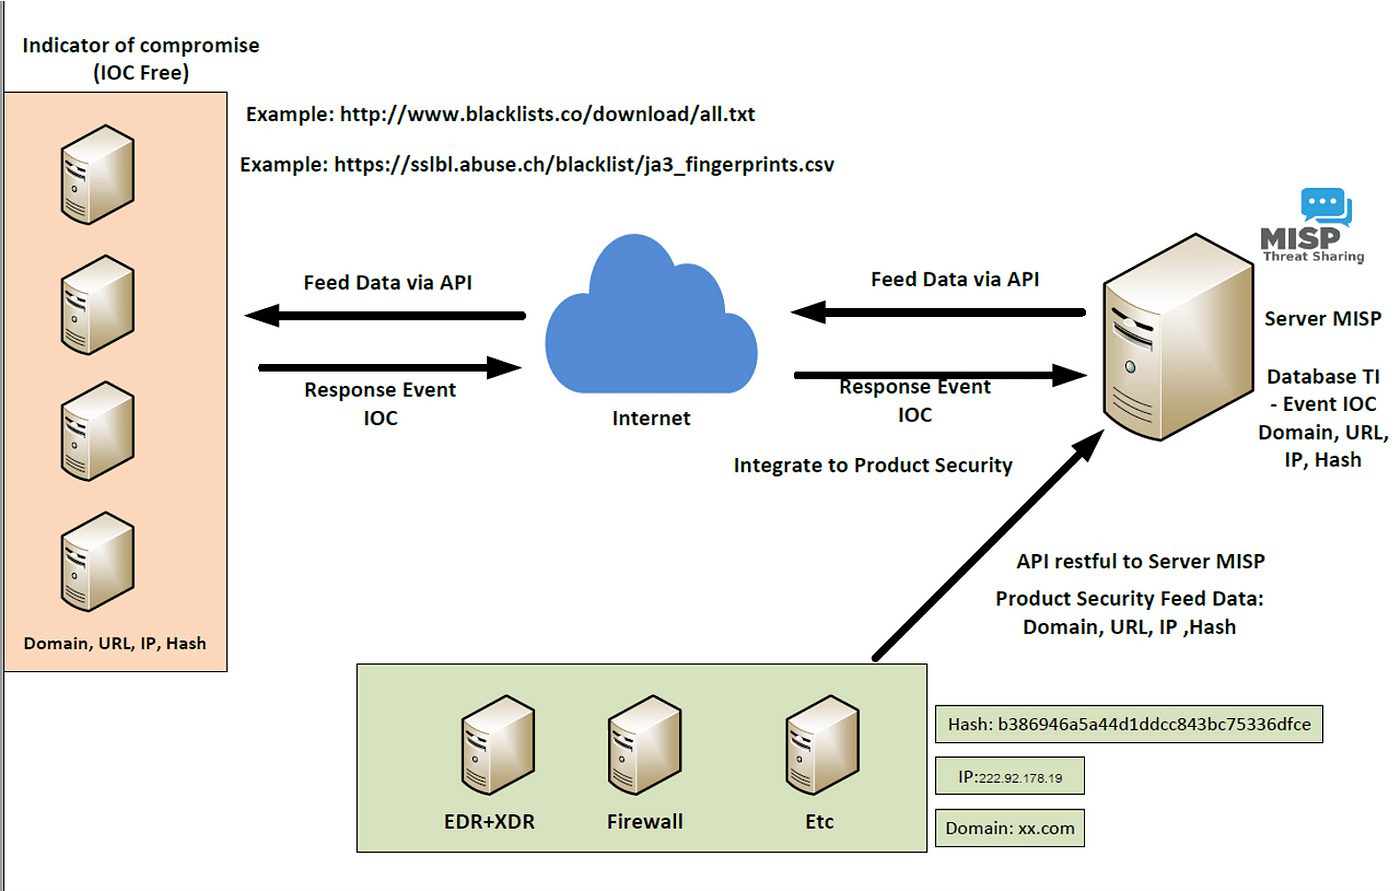
\includegraphics[width=0.9\textwidth]{assets/MispInfo.png}
    \caption[Récupération des IOC via l'API de notre instance MISP locale (source: \url{https://so-sonajaa.medium.com/misp-malware-information-sharing-platform-ep1-eea91df7415b})]{Récupération des IOC via l'API de notre instance MISP locale}\label{fig:MispInfo}
\end{figure}

\vspace{1em}

En ce qui concerne les sources publiques, si je n'ai utilisé que les deux "Feeds" fournis par défaut par le CIRCL\footnote{\url{https://www.circl.lu/doc/misp/feed-osint/}}\footnote{\url{https://www.botvrij.eu/data/feed-osint/}} lors de l'installation de l'instance, le travail que j'ai effectué permettra cependant l'intégration de sources supplémentaires à l'avenir.

\newpage

\begin{figure}[h]%
    \center%
\begin{lstlisting}[language=Python]
# Import PyMISP
from pymisp import PyMISP
# local misp credential
from conf.misp_conf import misp_url, misp_user_key, misp_verifycert

# source d'events "feeds" :
feeds = [
    "https://www.circl.lu/doc/misp/feed-osint/",
    "http://www.botvrij.eu/data/feed-osint/"
]
# Autres "feeds" potentiels :
#   "https://bazaar.abuse.ch/downloads/misp/",
#   "https://urlhaus.abuse.ch/downloads/misp/",
#   "https://osint.digitalside.it/Threat-Intel/digitalside-misp-feed/",

# Connexion avec l'instance MISP
misp = PyMISP(misp_url, misp_user_key, misp_verifycert, 'json')

# Recuperation des events depuis les "feeds"
download_events(feeds)

# Integration des events dans l'instance local MISP
import_events(misp)
\end{lstlisting}
{\small
    \textit{Télécharge les événements à partir des sources fournies et les importe dans notre instance locale. "download\_events(feeds)" la fonction qui télécharge les événements. "import\_events(misp)" celle qui les importe dans notre instance locale de MISP. \hyperref[chap:annexe3]{[A.3]}}
    }
    \caption[Enrichissement de l’instance locale de MISP en évènement]{Enrichissement de l’instance locale de MISP en évènement}\label{fig:GetEventsMISP}
\end{figure}

\vspace{1em}

La seule importation des évènements, publiés par ces deux sources au cours des années 2023 et 2024, suffit à remplir notre instance de dizaine de milliers d'événements pouvant chacun partager des centaines d'IOC.\\

En plus de ces événements, je récupère les IOC détectés par nos propres équipements (Firewall, Sonde, etc.) ou par nos partenaires et un autre script Python permet la transformation de ceux-ci en évènement MISP.\\

\newpage

\begin{figure}[h]%
    \center%
\begin{lstlisting}[language=Python]
# Import PyMISP et MISPEvent
from pymisp import PyMISP
# local misp credential
from conf.misp_conf import misp_url, misp_user_key, misp_verifycert

# Connexion avec l'instance MISP
misp = PyMISP(misp_url, misp_user_key, misp_verifycert, 'json')
event = MISPEvent()

# Creer un evenement sur l'instance local MISP
response = create_event(3, 1, 1, "AMSN Example event with network IOC for Suricata", {"category": 'Network activity', "type": 'domain', "value": 'Vilain.com', "comment": 'AMSN Test domain for Suricata rule generation'}, ["tlp:white", "Phising"])
\end{lstlisting}
{\small
   \textit{Créer un événement exploitable à partir des informations associées. "create\_event(...)" la fonction qui crée un événement à partir d'information fournie. \hyperref[chap:annexe3]{[A.3]}}
    }
    \caption[Création événement MISP]{Création événement MISP}\label{fig:CreateMispEvent}
\end{figure}

\vspace{1em}

Les événements créés et les informations qui y sont enregistrées ont été conçus pour être compréhensibles par les analystes du SOC-MC et pour être exportables sous la forme de règles Suricata de la même manière que \hyperref[chap3:genRulesEvents]{\textbf{\textit{les autres IOC}}}.

\newpage

\subsubsection{Sélection des IOC}
\vspace{0.5em}

\hyperref[chap3:mispEvents]{\textit{\textbf{Comme mentionné plus haut}}}, seule une minorité d'IOC peut être utilisée, en raison du choix des technologies de détection de l'Agence. Afin d'optimiser le poids de notre instance locale et sa vitesse de réaction aux requêtes API de mes scripts, j'ai créé un autre script qui nettoie automatiquement notre instance de tous les IOC que nous ne sommes pas en mesure d'utiliser.\\

\begin{figure}[h]%
    \center%
\begin{lstlisting}[language=Python]
# Import PyMISP et MISPEvent
from pymisp import PyMISP
# local misp credential
from conf.misp_conf import misp_url, misp_user_key, misp_verifycert

# Types d'IOC dont nous avons besoin
suricata_types = [
    'ip-dst', 'ip-src', 'domain', 'domain|ip', 'url', 'uri', 'hostname',
    'md5', 'sha1', 'sha256', 'sha512'
]

# Recuperation de tous les events de l'instance local
events = misp.search(controller='events')

# Interrogation des events et suppression des attributs incompatibles avec les donnees de Suricata
for event in events:
    event_id = event['Event']['id']
    misp_event = misp.get_event(event_id)
    
    for attribute in misp_event['Event']['Attribute']:
        if not is_suricata_compatible(attribute):
            # Suppression de l'attribut non compatible avec Suricata
            misp.delete_attribute(attribute['id'])
\end{lstlisting}
{\small
    \textit{Supprime tous les IOC qui ne font pas partie de ceux désignés dans la liste 'suricata\_types' de l'instance local MISP.}
    }
    \caption[Suppression des IOC inutiles]{Suppression des IOC inutiles}\label{fig:RemoveIOC}
\end{figure}

\vspace{1em}

En outre, j'utilise une fonctionnalité offerte par MISP, les "Decaying Models"\footnote{\url{https://www.misp-project.org/2019/09/12/Decaying-Of-Indicators.html/}} qui attribuent aux IOC une durée de vie en fonction de leur type et un score qui diminue au fil du temps.\\

\newpage

\begin{figure}[h]%
    \center%
    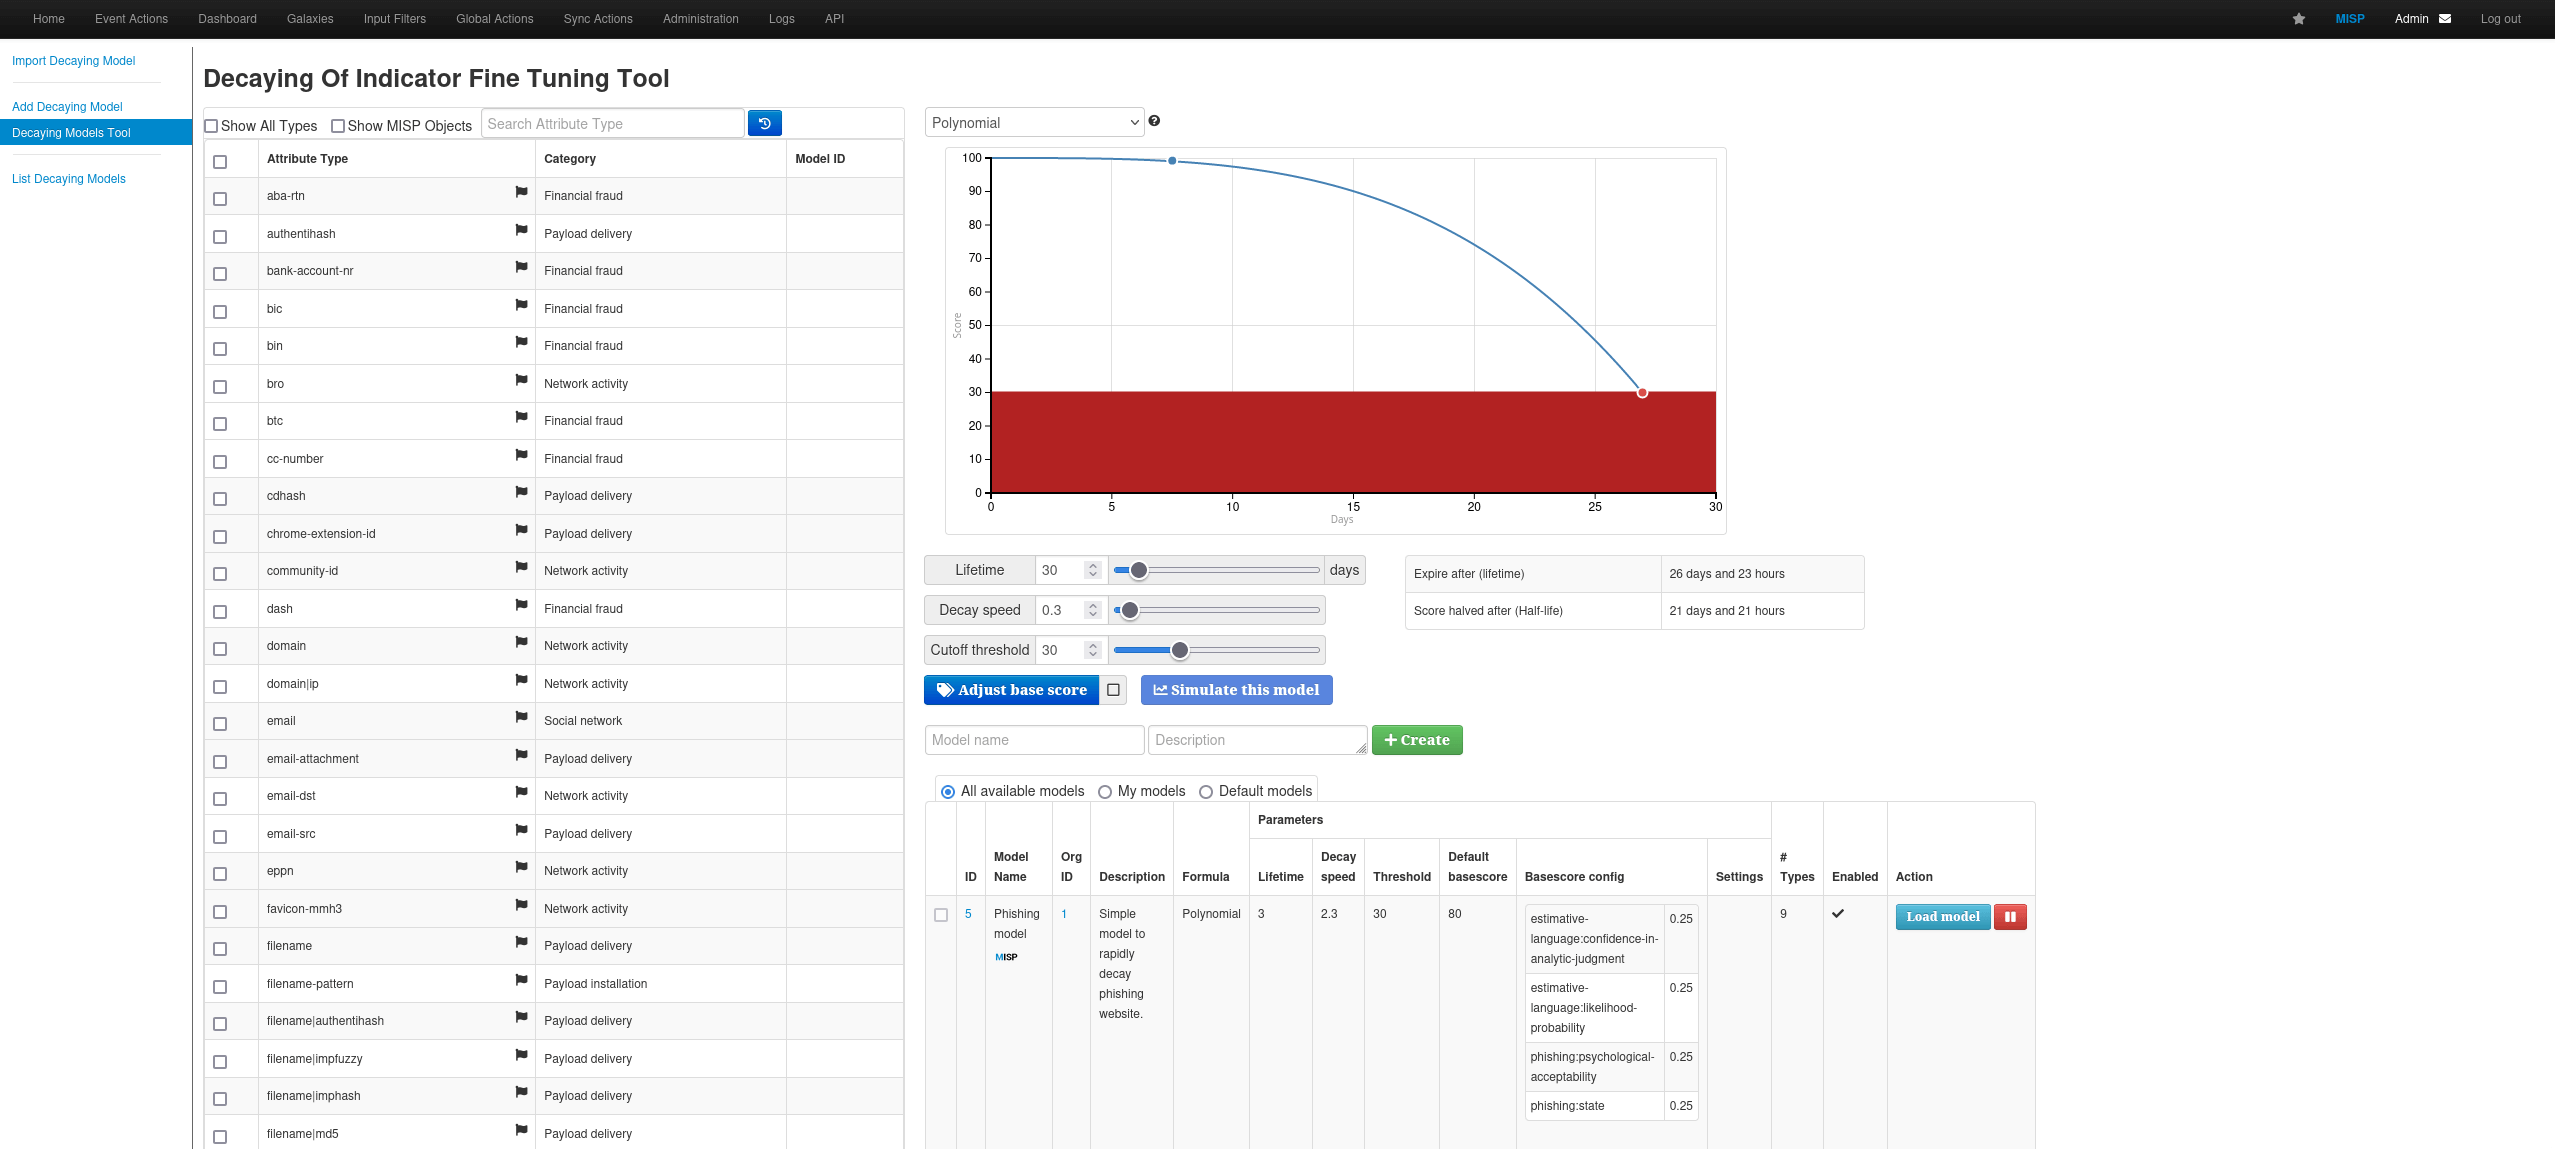
\includegraphics[width=1\textwidth]{assets/CaptureDecayingModel.png}
    \caption[Exemple de "Decaying Model" (source : capture d'écran de l'interface graphique de l'instance de test locale MISP)]{Exemple de "Decaying Models" (source : capture d'écran de l'interface graphique de l'instance de test locale MISP)}\label{fig:CaptureDecayingModel}
\end{figure}

\vspace{1em}

Pour l'instant, le modèle par défaut proposé par le MISP "NIDS Simple Decaying Model"\footnote{\url{https://github.com/MISP/misp-decaying-models/blob/main/models/nids-simple-model.json}} est utilisé sur l'instance. Les adresses IP, les noms de domaine et les URL ont ainsi une durée de vie de deux mois, après quoi les IOC en question sont considérés comme obsolètes (car la probabilité que ces IOC ne soient plus utilisés, par les acteurs malveillants détectés à l'origine, est trop élevée). \hyperref[biblio]{[2]}\\

À terme, l'AMSN souhaiterait travailler à la création de ses propres modèles d'obsolescence des IOC sur la base du retour d'information des analystes du SOC-MC et de ses partenaires.

\newpage

\subsubsection{Génération de règles à partir des IOC}
\label{chap3:genRulesEvents}
\vspace{0.5em}

Une fois que l'instance locale a été remplie d'événements et que les données ont été nettoyées, PyMISP offre la possibilité d'exporter directement les \textit{Attributes} des événements en règles Suricata.\\

\vspace{1em}

\begin{figure}[h]%
    \center%
\begin{lstlisting}[language=Python]
# Import PyMISP et MISPEvent
from pymisp import PyMISP
# local misp credential
from conf.misp_conf import misp_url, misp_user_key, misp_verifycert

# Prend tous les events et fabrique avec un fichier .rules exploitable
suricata_rules = misp.search(controller='events', return_format="suricata")
\end{lstlisting}
{\small
    \textit{Génère des règles de suricata à partir des IOC de tous les événements présents dans l'instance locale.}
    }
    \caption[Génération de règle Suricata depuis l'instance local MISP]{Génération de règle suricata depuis l'instance local MISP}\label{fig:CreateSuricataMISP}
\end{figure}

\vspace{1em}

Pour chaque attribut d'événement, une règle Suricata capable de détecter l'IOC de l'attribut est générée. Par exemple :\\

\newpage

\begin{figure}[h]%
    \center%
    L'IOC :\\
    \vspace{0.5em}
    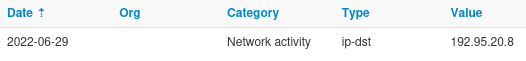
\includegraphics[width=0.9\textwidth]{assets/IP.png}
    \vspace{1em}
    \\Provenant de l'évènement :\\
    \vspace{0.5em}
    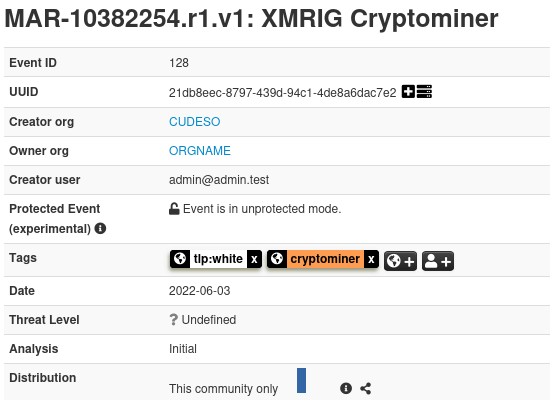
\includegraphics[width=0.8\textwidth]{assets/MispEventRule.png}
    \vspace{1em}
    \\Génère la règle :
    \begin{lstlisting}[language=bash]
alert ip $HOME_NET any -> 192.95.20.8 any (msg: "MISP e128 [] Outgoing To IP: 192.95.20.8"; classtype:trojan-activity; sid:2696602; rev:1; priority:4; reference:url,https://192.168.215.128/events/view/128;)
\end{lstlisting}
    
    \caption[Exemple de génération de règle Suricata par MISP (source : capture d'écran de l'interface graphique de l'instance de test locale MISP)]{Exemple de génération de règle Suricata par MISP (source : capture d'écran de l'interface graphique de l'instance de test locale MISP)}\label{fig:IP}
\end{figure}

\vspace{1em}

Les tests effectués avec le SOC-MC ont révélé que ces règles étaient fonctionnelles en l'état, mais qu'elles ne contenaient pas les informations contextuelles nécessaires pour comprendre et classer les alertes qu'elles généraient. Cela m'a conduit à créer un script supplémentaire pour reformater les règles générées par MISP. Pour ce faire, je n'ai modifié que deux variables dans la section \textit{options} des règles qui n'affectent pas leur capacité de détection :\\

\newpage

\begin{itemize}[itemsep=1em]
    \item[•] Soit la variable 'msg' (qui est une variable facultative utilisée pour donner des informations contextuelles sur la règle) en indiquant le nom de l'événement lié à la règle avec un lien vers l'événement sur l'interface graphique de l'instance MISP, à laquelle les analystes SOC peuvent accéder depuis leur poste de travail à l'aide de leur navigateur ;
    \item[•] Et la variable 'metadata' (qui est une variable optionnelle utilisée pour donner des informations supplémentaires à une règle) que j'ai complétée pour ajouter les 'Tags' de l'événement lié à cette règle.\\
\end{itemize}

\begin{figure}[h]%
    \center%
\begin{lstlisting}[language=Python]
# Prend tous les events
suricata_rules = misp.search(controller='events', return_format="suricata")

for rule in suricata_rules:
    ruleurl = re.search(r'reference:url,(.*?);', rule)
    if ruleurl:
        # On remplace le message original des regles (peu lisible et trop long) par un message simple renvoyant vers la pages MISP de l'Event
        rule = re.sub(r'msg: "(.*?)";', 'msg: "MISP event: ' + ruleurl.group(1) + '";', rule)
        # Ajout des tags de l'events
        rule = re.sub(r'metadata: "(.*?)";', 'metadata: tags ' + eventTags + '";', rule)
        new_lines.append('alert ' + rule)
\end{lstlisting}
{\small
    \textit{Modifie les variables des règles générées par MISP.}
}

\vspace{1em}
Règle après modifications :
\vspace{0.5em}
\begin{lstlisting}[language=bash]
alert ip $HOME_NET any -> 192.95.20.8 any (msg: "MISP Event : MAR-10382254.r1.v1: XMRIG Cryptominer https://192.168.215.128/events/view/128"; classtype:trojan-activity; sid:2696602; rev:1; priority:4; reference:url,https://192.168.215.128/events/view/128; metadata: tags tlp:white|cryptominer;)
\end{lstlisting}
    \caption[Modification des règles générées par MISP]{Modification des règles générées par MISP}\label{fig:ModifRulesMISP}
\end{figure}

\vspace{1em}

L'ajout du titre de l'événement présente l'avantage d'indiquer plus clairement aux analystes l'objectif de détection de la règle, et le lien vers l'interface graphique MISP leur permet de rechercher plus d'informations sur la règle directement sur MISP en cas d'investigation.\\ 

\newpage

L'ajout de "Tags" à l'événement fournit également des informations supplémentaires sur la règle, mais permet surtout de classer les règles en catégories, qui peuvent ensuite être utilisées pour créer des statistiques basées sur celles-ci, ou évaluer leur utilité en fonction des sondes sur lesquelles elles seront appliquées.\\

Une fois reformatées, les règles générées peuvent être directement ajoutées aux règles ingérées par \hyperref[chap3:section1]{\textbf{\textit{mon premier programme}}} pour être intégrées dans les sondes.

\vspace{1em}

\subsubsection{\textit{Note}}
Le développement de ce code a également pris environ un mois et demi, comprenant la rédaction de la documentation. L'instance de MISP mentionnée dans cette section a été installée et testée dans une section distincte du réseau interne avec des données de test. Les réactions de mon tuteur de stage et des analystes du SOC-MC sont positives quant au potentiel offert par cette instance locale, mais pour l'instant, elle n'est pas encore utilisée dans les processus actuels de l'Agence, dans l'attente de la planification du déplacement de la VM de l'instance sur le réseau de production.